\documentclass[12pt]{article}
% font size could be 10pt (default), 11pt or 12 pt
% paper size coulde be letterpaper (default), legalpaper, executivepaper,
% a4paper, a5paper or b5paper
% side coulde be oneside (default) or twoside 
% columns coulde be onecolumn (default) or twocolumn
% graphics coulde be final (default) or draft 
%
% titlepage coulde be notitlepage (default) or titlepage which 
% makes an extra page for title 
% 
% paper alignment coulde be portrait (default) or landscape 
%
% equations coulde be 
%   default number of the equation on the rigth and equation centered 
%   leqno number on the left and equation centered 
%   fleqn number on the right and  equation on the left side
%
\usepackage{graphicx}
\usepackage{geometry}
\usepackage{epigraph}
\usepackage{url}
\usepackage{fancybox}
\usepackage{textpos}
\usepackage{indentfirst}
\usepackage{rotating}
\usepackage{pdflscape}
\usepackage{listings}
\usepackage{tcolorbox}
\definecolor{light-gray}{gray}{0.95}
\usepackage{courier}
\usepackage{appendix}
\lstset{basicstyle=\footnotesize\ttfamily,breaklines=true,numbers=left}
%\usepackage{parskip}
%\setlength{\parskip}{\medskipamount}
\makeatletter
\newcommand{\@minipagerestore}{\setlength{\parskip}{\medskipamount}
\setlength{\parindent}{17pt}}
  \makeatother

\title{Reclaiming a Waveguide Switch -- An Adventure In 3D Printing}
\author{Matt Reilly  \\
	kb1vc \\
	}

\date{\today} 
% \date{\today} date coulde be today 
% \date{25.12.00} or be a certain date
% \date{ } or there is no date 
\begin{document}
% Hint: \title{what ever}, \author{who care} and \date{when ever} could stand 
% before or after the \begin{document} command 
% BUT the \maketitle command MUST come AFTER the \begin{document} command! 
\maketitle

\begin{abstract}
  A simple and somewhat reliable 3D printer can now be had for about \$200.
  While such a printer can help create new widgets and interesting objects, 
  it also affords an opportunity to refurbish or even reclaim equipment that
  may be lying around the shop in need of a hard-to-get part. This is the
  story of one such project that replaced a burned out actuator with a
  R/C model airplane servo and an Arduino controller.  All for 
  less than the cost of a replacement unit on eBay.
\end{abstract}

\setlength{\epigraphwidth}{0.8\textwidth}
\epigraph{[Engineering] is the art of doing that well with one dollar,
  which any bungler can do with two after a fashion.}{Arthur M. Wellington \\
  ``The Economic Theory of \\
  the Location of Railways''}


%\tableofcontents % create a table of contens 



\section{Introduction}

Most engineers read Mr. Wellington's dictum with great pride
that their training has placed them above the run-of-the-mill bungler.
I know that I do.
When it comes to mechanical engineering, however, I am a bungler.
In this case Wellington provides encouragement: it {\em may} be possible
to do what an expert can do for just twice the cost!

And so began my adventures in 3D printing.

\begin{figure}[htb]
  \centering
  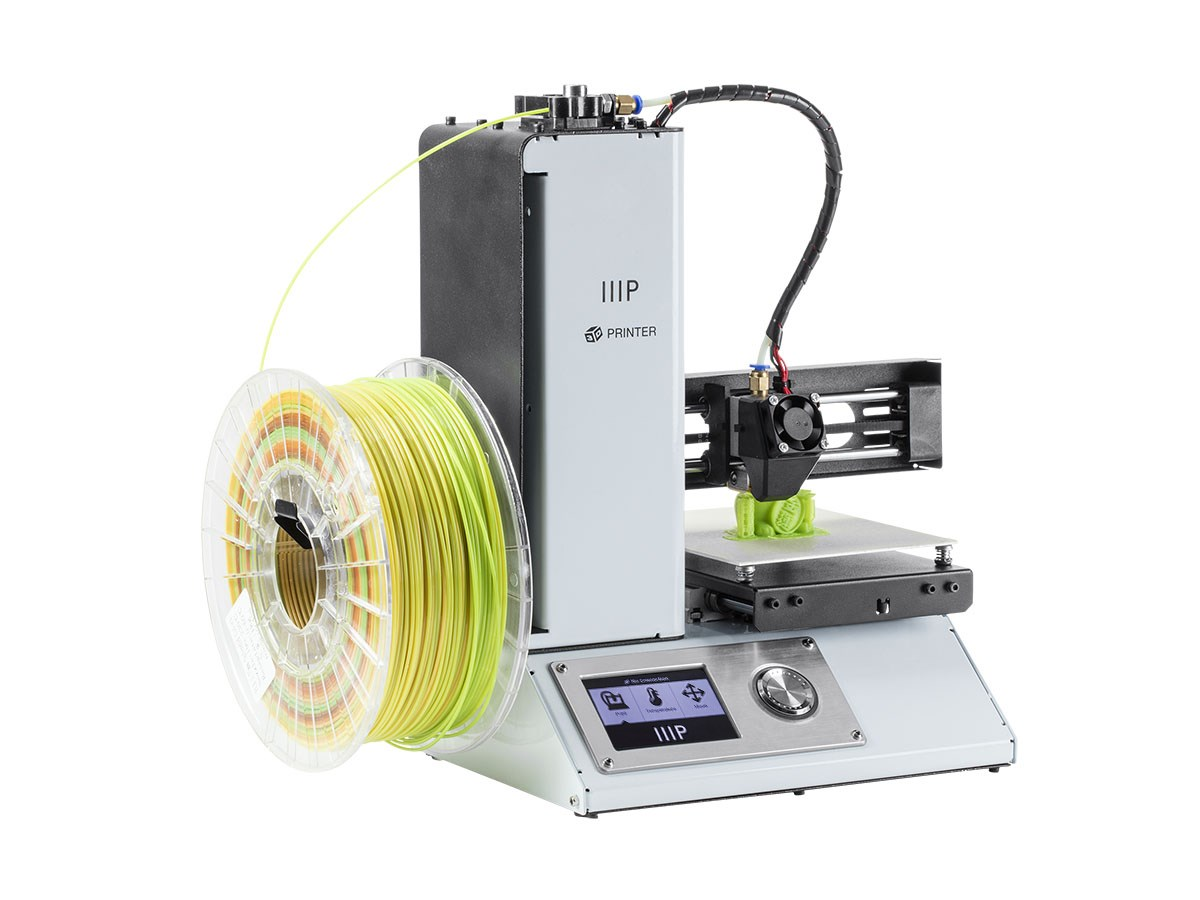
\includegraphics[width=0.6\textwidth]{MiniSelect3DPrinter.jpg}
  \caption{\label{f_printer}The Monoprice Mini Select 3D Printer}
\end{figure}


\section{Starting Simple}

This article is about reclaiming a WR75 waveguide switch by adapting
a common hobby airplane servo to function as the positioner. It comprises
a set of plastic parts to couple the servo to the waveguide slug,
and an Arduino controller.

But before we dive in to the construction of the waveguide switch positioner,
it may help to look at a much simpler 3D printing project.

Quite a while back, I bought an HP6289A DC power supply at a hamfest.
It was a real find, but at some point in its checkered past it had
been dropped on its face.  The fall shattered the two fine adjustment
knobs.  These were concentric with the coarse adjustment knobs on two
shafts: one for voltage and the second for current.  For years, the
absence of the knobs was no great annoyance. But one night I decided
that making replacements might be a short and simple project.

In the old days, I'd have scavenged in the scrap box for a nylon rod
or perhaps even an aluminum bar, mounted it in the lathe, turned it down,
bored out the hole for the shaft, tracked a few pieces of swarf while
passing through the living room, found that it didn't quite fit, tried
again... In total, I'd have spent a happy hour or two all together from
looking for bar stock, to vacuuming swarf out of the carpet.

This kind of project really points out the virtues of an inexpensive
3D printer.  No great precision is needed, and the cost of a mistake
is a small amount of material and time waiting for the
printer to finish.\footnote{The knobs were very small and simple. They
  took about 15 minutes to print. Typical
  print times for most interesting components can range from one to
  eight hours.}
It took two tries to get the design right. Had I
been paying attention, it could have been right the first time.
But having the printer in the shack
meant that I got through two iterations in less than an hour.
And no metal waste got stuck in the carpet. 

\begin{figure}[tb]
  \centering
  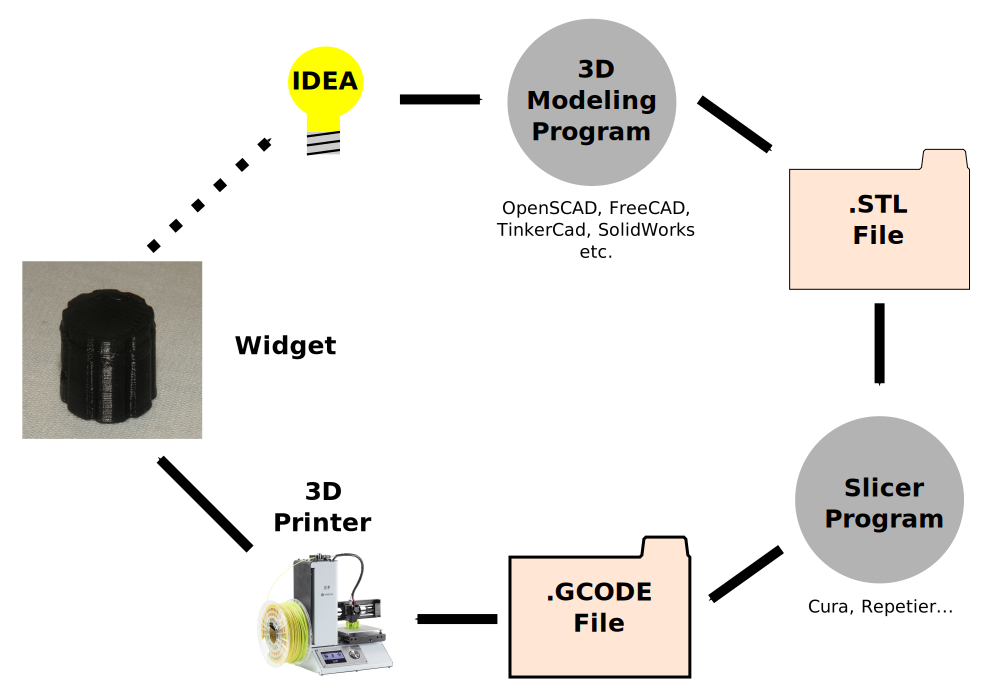
\includegraphics[width=0.8\textwidth]{Idea2Print.pdf}
  \caption{\label{f_3d_process}Printing in 3D from Idea to Widget}
\end{figure}

Figure \ref{f_3d_process} shows the path to a printed widget.  The
process starts with an idea which is reduced to a 3D model using
OpenSCAD to produce a stereo-lithography (STL) file.  The STL file
describes the object as a set of surfaces that bound a solid volume.
This is converted into instructions that move a 3D printer's extruder
and deposit the hot filament into the desired shape. The conversion
program is called a ``slicer'' because it converts the solid model
into a series of two dimensional planes that are deposited in layers
by the extruder.  The printer for this project is a Monoprice Mini
Select from \url{https://www.monoprice.com/} shown in Figure
\ref{f_printer}.The retail price is \$199. The quality of output from
the printer is variable, but compares favorably with much more
expensive printers. Though the manufacturers claim it can print in a
variety of materials, it works best with PLA, and not at all well with
ABS.

\begin{figure}[tb]
  %\caption*{About Materials}
\fbox{%
  \begin{minipage}{\textwidth}
\begin{tcolorbox}[colback=gray!35]
    \begin{center}
      {\bf About Materials}
    \end{center}
    ABS (Acrylonitrile Butadiene Styrene, for those keeping score at
    home) is the familiar plastic that shows up in instrument cases,
    helmets, canoes, and waste pipes.  It can be machined, and can
    even be given a glossy finish with exposure to acetone vapors.  It
    is, however, difficult to print on an economy-priced printer.

    PLA (Polylactic Acid) is most often found in disposable drinking
    cups.  It is often used where its potential for recycling is
    important. Some would claim that it is ``biodegradable'' as there
    are bacteria that eat it.  This has caused concern that
    widgets built with PLA might disintegrate while in use.  However,
    the process of breaking down PLA requires a fair amount of
    pressure and/or heat.  Relative durability for PLA can be assured
    by avoiding installations in compost heaps or animals.  Though my
    shack is something of a mess, it has not yet achieved the status
    of ``compost heap.''
    \end{tcolorbox}
\end{minipage}}
\end{figure}

Making the replacement knobs began with a model in OpenSCAD. OpenSCAD
scripts describe three dimensional things by building them
up from simple solids like cubes, spheres, cylinders, and cones.
Shapes can be added or subtracted, so that a simple knob can be
described as an outer cylinder minus an inner cylinder.  The inner
cylinder is the hole for the salvaged shaft collar. OpenSCAD allows the designer to
view an object on screen and to translate scripts into STL (stereo-lithography)
files for later processing. (The description language and the OpenSCAD
editor are described at \url{http://www.openscad.org/}.)

As this project aimed to replace the rather fancy HP original components,
the knobs had a bit of a taper to them, and a hole in the side for a
retaining screw. Figure \ref{f_openscad} is a screenshot of an OpenSCAD
session showing the knob. The model file is shown in Figure \ref{f_knob_list}.

\begin{figure}[htbp]
  \lstinputlisting{HP6289_inner.scad}
  \caption{\label{f_knob_list}OpenSCAD Model of Replacement Knob}
  \end{figure}

OpenSCAD scripts can follow many forms, but my own approach is to put
all of the important dimensions at the top of the file, and then
describe each feature of the object hierarchically.  For the knobs,
it was useful to describe the shaft diameter (line 2), 
the minimum wall thickness (line 3), the length of the knob (line 5),
the set screw (lines 6 and 7), and the depth of cut for the knurling (line 8).

The knob itself comprises a body, a hole for the shaft collar, a hole
for the setscrew, and the knurling.  These are all assembled in the
last module {\tt HP6289\_Inner}. The module is actually expanded in
lines 39 and 40.  OpenSCAD's default unit is the millimeter, but I
tend to measure in imperial units, so line 39 translates from inches
to mm.

\begin{figure}[tb]
  \centering
  \begin{minipage}[b]{0.4\textwidth}
    \centering
    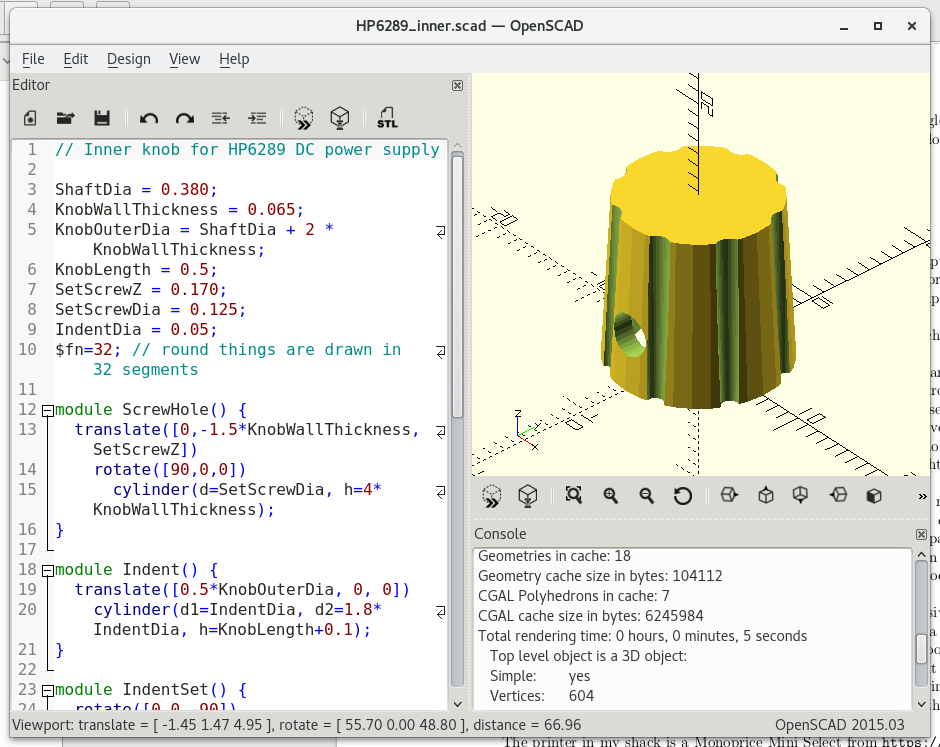
\includegraphics[width=\textwidth]{PSKnob_OpenSCAD.png}
    \caption{\label{f_openscad}OpenSCAD session showing replacement knob}
  \end{minipage}\qquad
  \begin{minipage}[b]{0.4\textwidth}
    \centering
    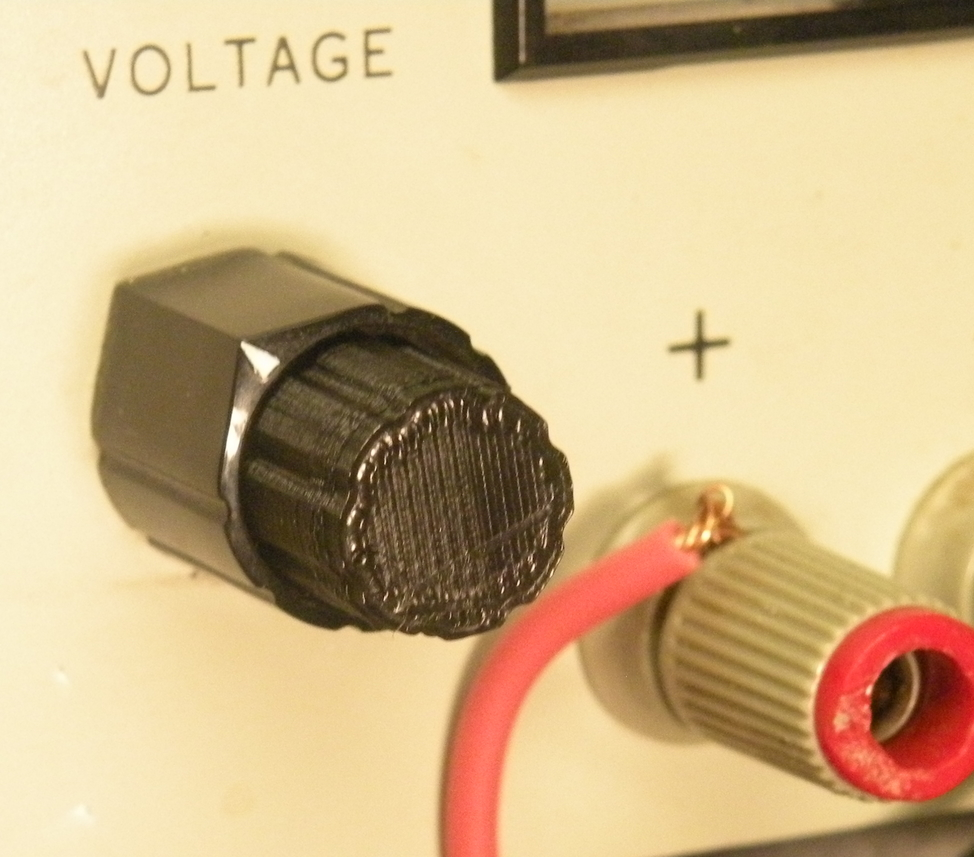
\includegraphics[width=\textwidth]{SmallKnob.jpg}
    \caption{\label{f_knobs_on_box}Replacement power supply knob in its new home}
  \end{minipage}
\end{figure}


A pleasant evening of head-scratching and printing produced the two
knobs shown in Figure \ref{f_knobs_on_box}.  The result won't be
mistaken for original parts, but the power supply is a tool in a
workshop, not a museum display.

\section{The Waveguide Switch}

Years ago I bought a WR75 waveguide switch to use in a 10GHz transceiver.
The actuator was a pair of coils mounted to a shaft, and surrounded by
a pair of permanent magnets.  The shaft moved a slug inside the switch.
The switch functioned well for about ten years, but finally gasped its last
when one of the coils melted. (It appears that the microswitch that
handled the latching function may have gotten stuck.)

I disassembled the unit to complete the forensic investigation.  A short
examination convinced me that it was toast.  Rewinding the armature was
not all that appealing, and I'd recently acquired some good microwave relays,
so the broken shards sat on the shelf for a year or so, until I found the body
of the switch while looking for something else. The notion hit me that I
could replace the coil/magnet assembly with a R/C model airplane servo.
These were inexpensive and easy to control with an Arduino microcontroller
and a few lines of code.

Figure \ref{f_wg_switch_orig} shows a switch similar to the unit I started
with.\footnote{Thanks to Dudley Lab \url{http://www.dudleylab.com/surplus6.html} for the image.}  
The ``finished'' unit is shown in Figure \ref{f_wg_switch_new}. 

\begin{figure}[tb]
  \centering
  \begin{minipage}[b]{0.4\textwidth}
    \centering
    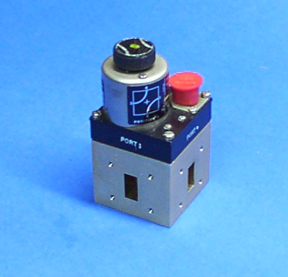
\includegraphics[width=\textwidth]{wr-90-s1.jpg}
    \caption{\label{f_wg_switch_orig}Original switch (+/-)}  
  \end{minipage}
  \begin{minipage}[b]{0.4\textwidth}
    \centering
    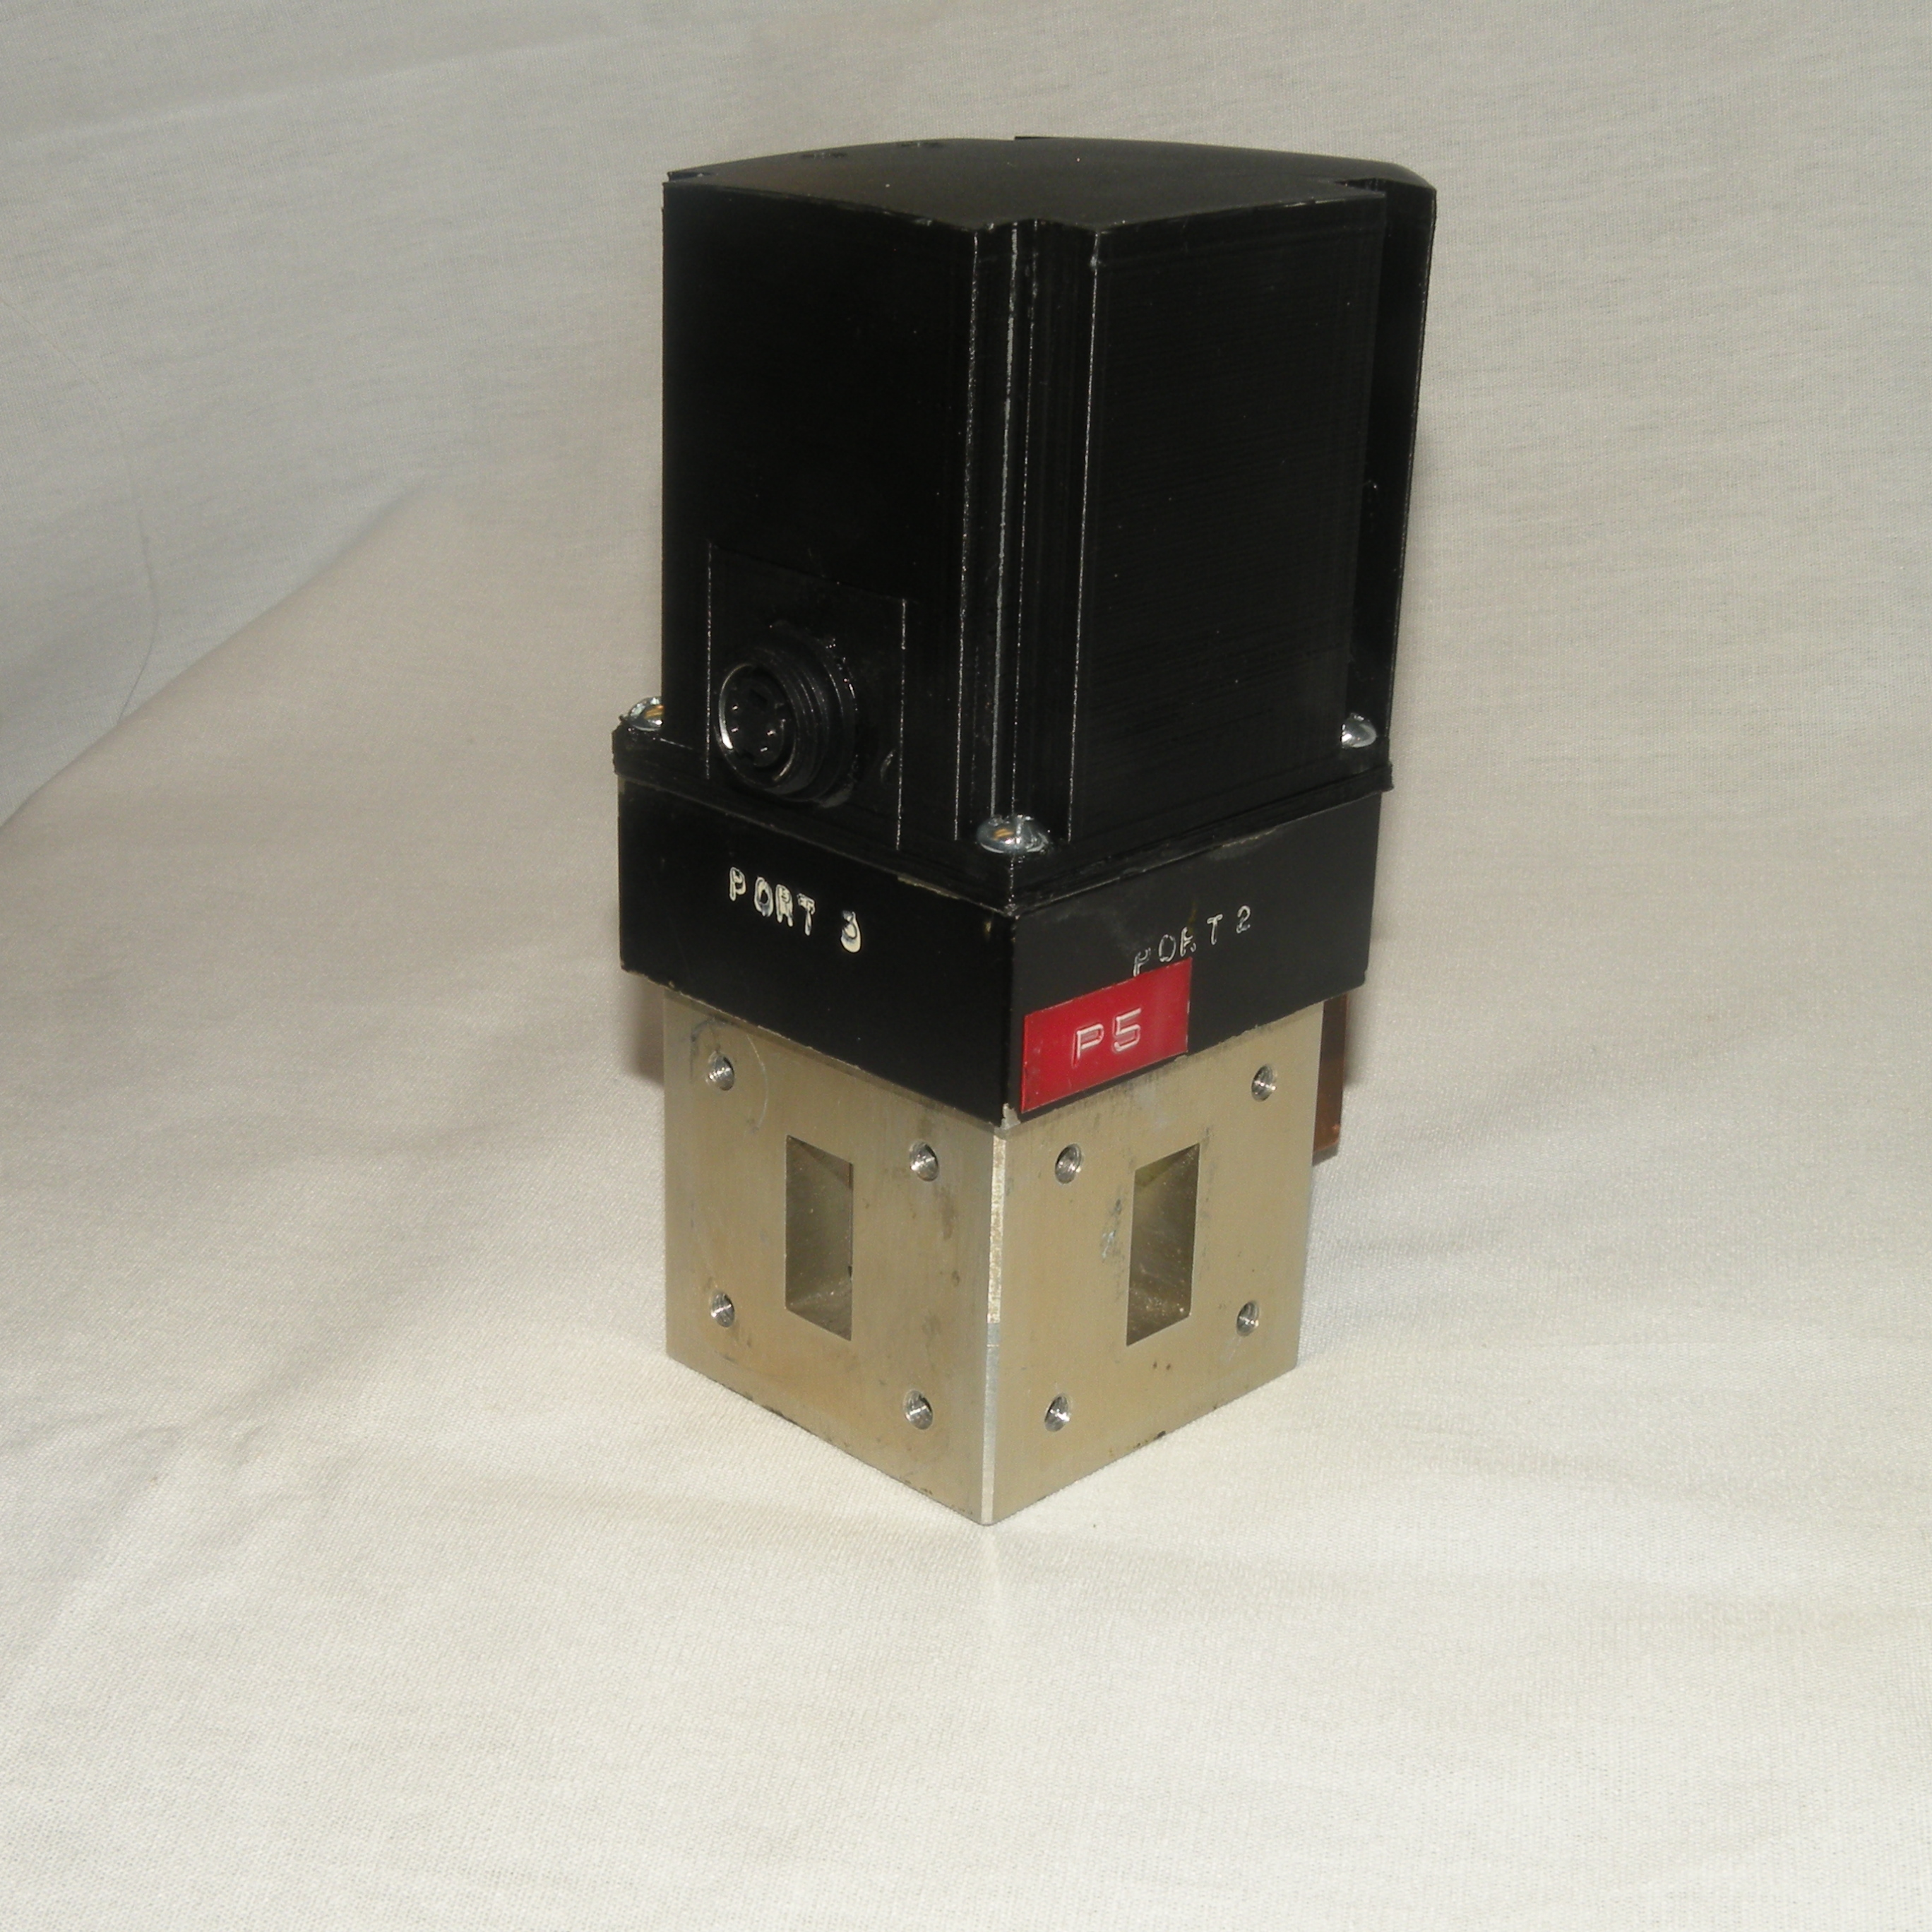
\includegraphics[width=\textwidth]{WGFinal.jpg}
    \caption{\label{f_wg_switch_new}Reclaimed unit}      
  \end{minipage}
  \end{figure}


The trick was mating the servo to the keyed shaft of the waveguide switch,
and sensing the position of the switch.  A typical servo is not very
accurate. The control mechanism is a pulse train where the angular position
of the servo is more-or-less proportional to the pulse width.  The more-or-less
part meant that any positioning mechanism would need some kind of feedback
or other scheme to make sure the waveguide slug was aligned with the input
and output ports.

As an amateur bungler, it took a number of experiments before a
reasonably reliable method for positioning the slug was found. Figure
\ref{f_trial_and_error} shows 30 or so parts that were printed on the
way to a working design.  The total cost for all the material used in
the trials was less than \$10.

\begin{figure}[tb]
  \centering
  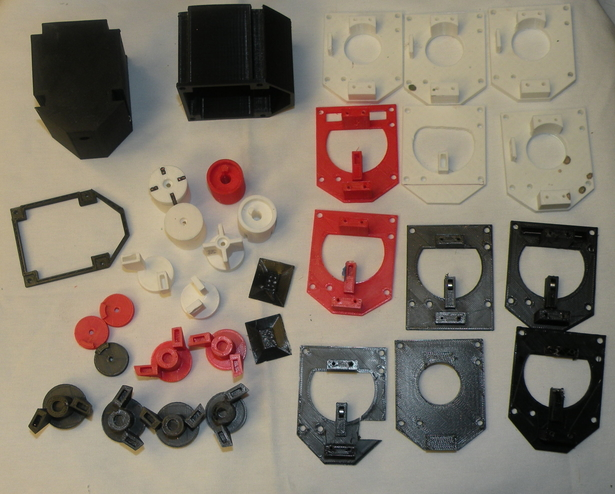
\includegraphics[width=0.8\textwidth]{TrialAndError1.jpg}
  \caption{\label{f_trial_and_error}Trial and Error Parts}
\end{figure}

\begin{figure}[thb]
\centering
    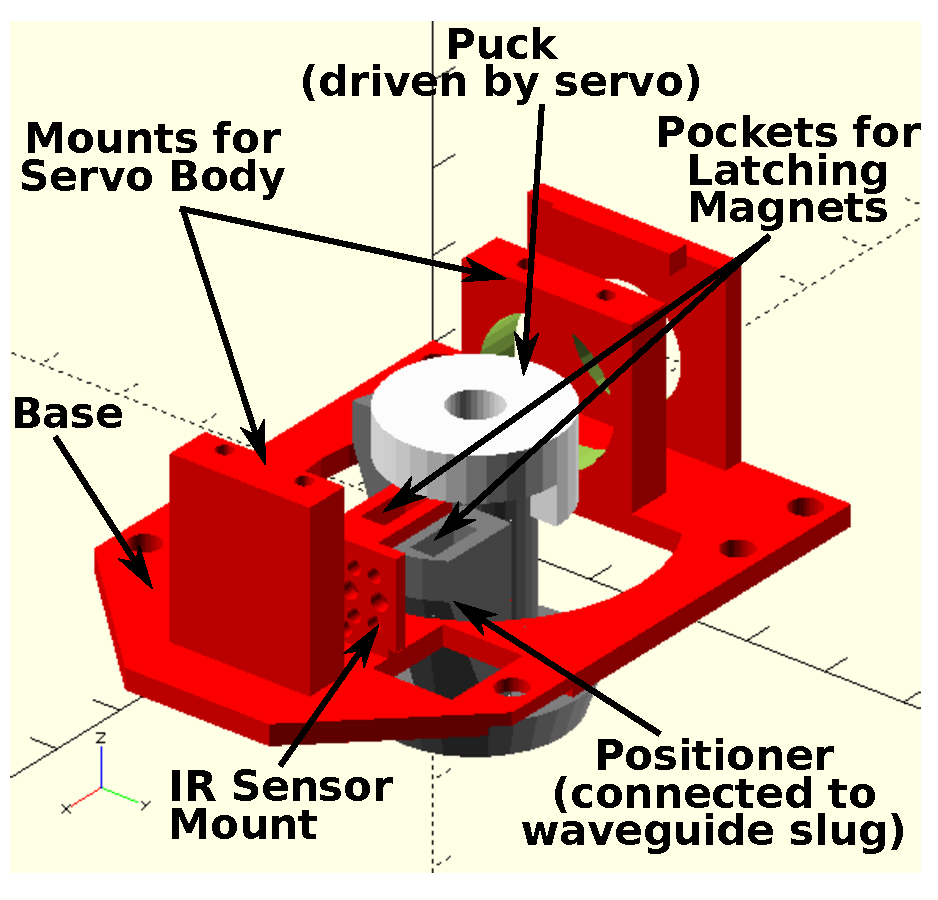
\includegraphics[width=0.7\textwidth]{AssemblyView.pdf}
    \caption{\label{f_expview}The Positioning Mechanism (minus the servo)}  
\end{figure}


Positional accuracy is established with a mechanical stop at each
position as shown by the assembly view in Figure \ref{f_expview}. The
metal slug in the waveguide switch itself is coupled to a positioner
(dark gray) that is pushed by the puck (white) into the RX or TX
position, and stopped by a protrusion on the base (red). Each vane in
the positioner has a pocket for a small 6mm rare earth magnet. These
are captured by a magnet in the pocket in the stop block on the
base. The servo needs only to push the positioner vane to the stop and
may then recede. The magnets hold the positioner (and the waveguide
slug) in place until the servo is commanded to switch modes.  As a
``fail-safe'' mechanism, the controller will not assert its TX\_EN
output line until an infra-red position sensor detects that the
positioner vane is in place against the stop block.  On deassertion of
the PTT line, the controller maintains the servo position against the
positioner until a similar IR sensor on the RX side detects that the
positioner is in place against the stop block on the RX side.

The servo is controlled with an Arduino Pro Mini (available from
Sparkfun at \url{https://www.sparkfun.com/products/11113}) on a module
that provides level translation and limited isolation for the PTT
input line and the TX\_EN output line. (See Appendix \ref{a_controller_module}
for the schematic.)

The OpenSCAD files, the schematic and PCB layout, and Arduino code are
all available for use under the ``BSD 2-clause Simplified License'' that
allows commercial use, modification, distribution, and private use.
The design package can be downloaded from github at \url{https://github.com/kb1vc/waveguide-switch}.

\section{Building the Switch}

It would be surprising if anyone actually built exactly this module,
as it will likely require some modification for each type of waveguide
switch.  Nevertheless, the assembly instructions are provided here to
serve as a starting point for others. Assembly directions are tedious
and make for lousy reading.  You've been warned. 

\subsection{The Arduino Controller}

The first version of the Arduino based controller assumed ground-to-actuate
input for the PTT switch that was routed directly to the microcontroller.
(See the schematic in Appendix \ref{a_controller_module}.)
This is a really bad idea, so revision B will have some protection on this
input to isolate the microcontroller from potentially damaging voltages on the
PTT line and to provide some RF decoupling.
The REV A modules are available from OSH Park at \url{https://oshpark.com/shared_projects/Da0N0VIn}.
REV B is ``in progress.''

Assembly of the controller is straightforward, though almost all the components
are surface-mounted. The Pro Mini is soldered to the module as a daughter card.
The Pro Mini is availble in both 3.3V and 5V versions.  This controller uses the
5V model, as this tends to be better suited to driving an RC servo.

Once assembled, the controlling sketch may be downloaded into the module using a
USB to serial adapter from Sparkfun. (\url{https://www.sparkfun.com/products/9716})

The sketch is found in the design package under {\tt ../arduino/TRSwitchSleep}
and its current version is shown in Appendix \ref{a_sketch}. 
This sketch senses changes on the PTT input and activates the servo.
The servo is driven to its limit until the IR sensors mounted on the base indicate
that the positioner vane is pushing against the stop block. 
The TX enable output line is asserted {\em only} after the IR sensor detects
that the positioner is in the TX position.  The TX enable line is deasserted
(floats) as soon as the microcontroller detects a rising edge on the PTT input.
The sketch places the microcontroller in sleep mode between switching events to
reduce RF noise caused by its internal (and rather dirty) oscillators. 

\subsection{The Mechanical Bits}

The 3D printed parts for the switch are all described in a single
OpenSCAD file.  However, most small 3D printers will need to print
the lid and base parts separately, as they take up a fair amount
of room on the printer's platform.
To print the components:
\begin{enumerate}
\setlength\itemsep{0em}
\item Use OpenSCAD to generate an STL file (called {\tt WGSwitch.stl}) from
  the {\tt WGSwitch.scad} source file.
\item Open the {\tt WGSwitch.stl} file in Cura
\item Click MB3 on the model and select ``Split object into parts.''
  This will separate the four parts.
\item Delete the lid and the  base.
\item Save the gcode file as {\tt WGSwitchSmall.gcode}.
\item Quit Cura, then repeat steps 2 and 3.
\item This time delete all the parts except the base.
\item Save the gcode file as {\tt WGSwitchBase.gcode}.
\item Quit Cura, then repeat steps 2 and 3.
\item Delete all the parts except the lid.
\item Flip the lid over so that its open part faces up.
\item Save the gcode file as {\tt WGSwitchLid.gcode}.
\item Copy each of the gcode files to your 3D printer.
\item For best results, print the all components in black.
  At a minimum, the positioner and the base must be printed
  in a color that does not reflect IR well.
  \end{enumerate}

It would be a very bad idea to make this your {\em first} 3D printing
experience, as every printer requires a little fiddling and some
occasional attention.  The typical 3D printer is not nearly as
reliable as a 2D inkjet printer.

\begin{figure}[tb]
  \centering
  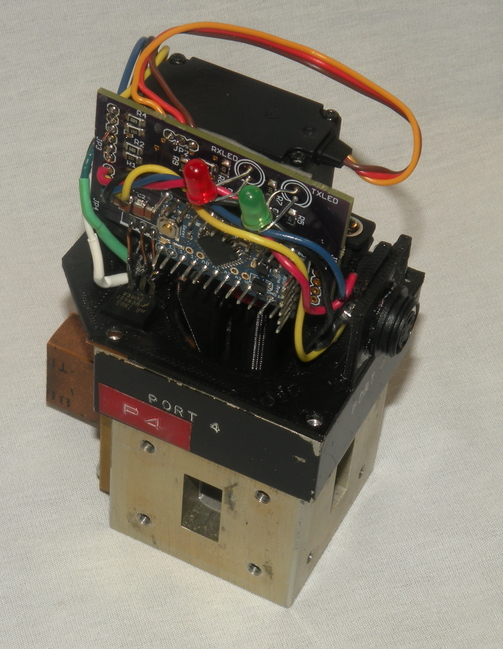
\includegraphics[width=0.5\textwidth]{BareModule.jpg}
  \caption{\label{f_naked_switch}The Controller, Servo, and Sensors}
\end{figure}


Once the parts have been printed, they should be ``tidied up'' with
a sharp knife here and there.  
The switch controller, {\em sans} lid, is shown in Figure \ref{f_naked_switch}.
Assembly is fairly straightforward.

\begin{enumerate}
\setlength\itemsep{0em}  
\item Mount the round puck on the shaft of the RC servo. Rotate the
  servo so that the shaft is at its midpoint position. Then align
  the key on the puck so that it is closest to the midpoint of the
  two mounting holes nearest the servo's shaft.
\item Mount the positioner onto the waveguide slug.
\item Insert two of the rare-earth magnets into the slots in
  the positioner, making sure the magnets are both facing with
  their poles in the same direction.
\item Place the base onto the waveguide switch body, lining up
  the locator and screw holes. Insert the LM7805 voltage regulator
  into the slot in the base. Ensure that the positioner vanes
  straddle the stop block in the base. Fasten the base to the
  switch body with four screws.
\item Insert a magnet into the slot in the base, making sure
  it is oriented so that it attracts each of the vanes in turn.
\item Glue the two IR proximity sensors into the base using
  a two-part epoxy.
\item Wire the IR sensors, the servo, and a 4 pin DIN connector
  to the controller module.
\item Fasten the controller to the side of the servo with
  double sided tape.
\item Paint a small reflective stripe on each of the vanes of the
  positioner, as shown in Figure \ref{f_positioner_stripe}.
  These will improve the reflectivity of the block. 
\item Glue the 4 pin DIN socket into the hole at one end
  of the base.
  \item Carefully stuff all that into the lid. 
  \end{enumerate}


\begin{figure}[tb]
  \centering
  \includegraphics[width=0.5\textwidth]{ReflectiveStripes.pdf}
  \caption{\label{f_positioner_stripe}Reflective Stripes on the Positioner Vanes}
\end{figure}

\begin{figure}[tb]
  %\caption*{About Materials}
\fbox{%
  \begin{minipage}{1.1\textwidth}
\begin{tcolorbox}[colback=gray!35]
    \begin{center}
      {\bf Drawing in 3D}
    \end{center}
There are lots of choices for preparing 3D models
for printing.  I prefer to use open source software.
Of the open source choices, I've used two:  FreeCAD
and OpenSCAD. 

FreeCAD is an open source alternative to the traditional
3D CAD suites like SolidWorks.  The interface and
the behavior will be familiar to users of the commercial
tools.  It provides a rich set of ``workbenches'' that
assist in creating parts, assemblies, and 2D drawings.
It is under active development, and has a support community.

OpenSCAD uses a script based approach to create constructive
solid geometry  models.  It is extremely powerful, and capable
of describing just about any physically realizable shape.

I started in 3D printing as a FreeCAD user.  It allowed me to
build boxes, knobs, and robot parts. However, I found that making
changes to a design was hit-and-miss.  The data structures that
FreeCAD used often made it impossible to move a hole a few mils,
or change the angle between two slabs.  After a particularly
aggravating episode where  several hours of work had to be
discarded because a hole was in the wrong place, I abandoned FreeCAD.

OpenSCAD encourages a cut-and-try approach that allows
easy modification.  The learning curve can be quite steep for
users who have never written a program before, but not insurmountable.

A third option offers a graphical approach to constructive solid geometry. 
Many elementary schools are using Tinkercad (\url{https://www.tinkercad.com})
to introduce students to 3D printing. Tinkercad runs in a web browser, but
allows the user to create models and download them for printing on a
3D printer. 
    \end{tcolorbox}
\end{minipage}}
\end{figure}

\clearpage
\section{Final Thoughts}


The arrival on the market of
an inexpensive 3D printer, and the well established Arduino
culture have given hams a new set of tools.  Experiments are
cheap and take far less time than traditional machine-shop
ventures. The project described here was done over a few
widely spaced weekends, despite the dozens of experiments
and refinements along the way. 

Building it was fun. The trial-and-error-and-error approach
took advantage of the low cost of each print.
The CAD tools allowed progressive refinement.
The minimal investment for each design iteration meant
that ``throw it out and start over'' was always an option.
The printer produced a usable device. And the
tools are available to any bungler.

\clearpage

\begin{appendices}

\section{\label{a_sketch}The Controller Arduino Sketch}
\lstinputlisting{../arduino/TRSwitchSleep/TRSwitchSleep.ino}

\clearpage
\newgeometry{top=1cm,bottom=1cm,left=1cm,right=1cm}
\section{\label{a_controller_module}The Servo Controller Module}
\begin{figure}[h] 
  \centering
  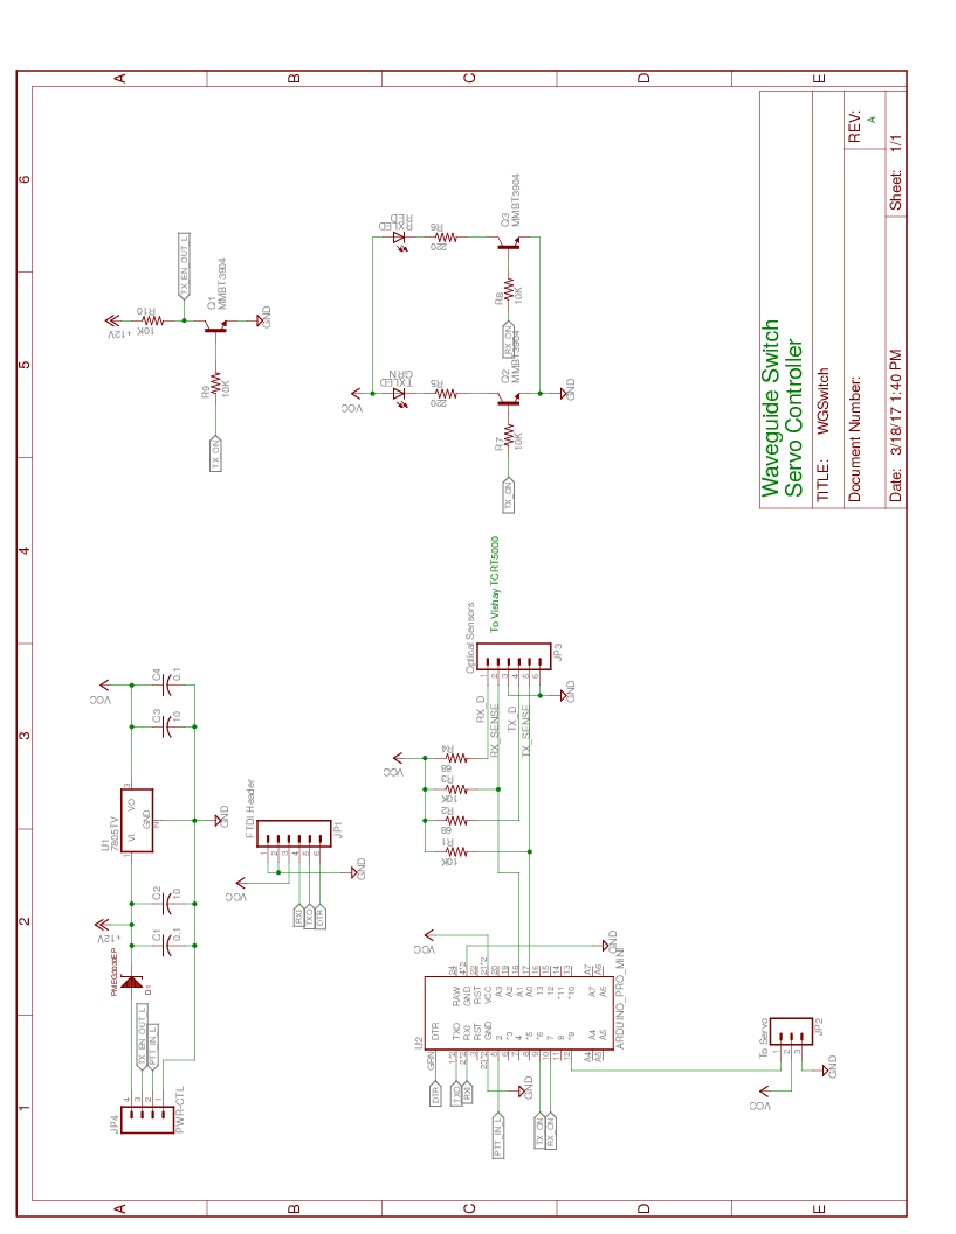
\includegraphics[width=0.75\linewidth,keepaspectratio]{WGSwitch.pdf}
\end{figure} 


%%\newpage
%%\newgeometry{top=1cm,bottom=1cm,left=1cm,right=1cm}
%%\section{\label{a_controller_mdoule}The Servo Controller Module}
%%
%%\begin{landscape}
%%\includegraphics[width=0.6\linewidth,keepaspectratio]{WGSwitchSchematic.pdf}
%%  \end{landscape}
%%\restoregeometry


\end{appendices}
\end{document}

